% !TeX program = pdflatex
% !TeX encoding = UTF-8
% !TeX spellcheck = pt_BR
\documentclass[
  article,
  11pt,
  a4paper,
  english,
  brazil,
  sumario=tradicional]{abntex2}
\usepackage{lmodern}			% Usa a fonte Latin Modern
\usepackage[T1]{fontenc}		% Seleção de códigos de fonte.
\usepackage[utf8]{inputenc}		% Codificação do documento (conversão automática dos acentos)
\usepackage{indentfirst}		% Indenta o primeiro parágrafo de cada seção.
\usepackage{nomencl} 			% Lista de simbolos
\usepackage{color}				% Controle das cores
\usepackage{graphicx}			% Inclusão de gráficos
\usepackage{microtype} 			% Melhorias de justificação
\usepackage{csquotes}			% Aspas e citações mais simples
\usepackage{booktabs}			% Tabelas mais profissionais

% ---
% Pacotes de citações
% ---
\usepackage[brazilian,hyperpageref]{backref}	 % Paginas com as citações na bibliografia
\usepackage[alf]{abntex2cite}	% Citações padrão ABNT
% ---

% ---
% Configurações do pacote backref
% Usado sem a opção hyperpageref de backref
\renewcommand{\backrefpagesname}{Citado na(s) página(s):~}
% Texto padrão antes do número das páginas
\renewcommand{\backref}{}
% Define os textos da citação
\renewcommand*{\backrefalt}[4]{
  \ifcase #1 %
  Nenhuma citação no texto.%
  \or
  Citado na página #2.%
  \else
  Citado #1 vezes nas páginas #2.%
  \fi}%
% ---

% Para fórmulas matemáticas
\usepackage{amsmath}
\usepackage{amssymb}
\usepackage{mathtools}

% Para setas usadas em fórmulas dos grafos
\usepackage{MnSymbol}

% Diretório padrão para figuras
\graphicspath{ {images/} }

% Permite colocar figuras lado a lado ou
% fazer posicionamentos arbitrários
\usepackage[lofdepth,lotdepth]{subfig}

\hypersetup{
  %hidelinks,   % Comente aqui para exibir os links
  colorlinks, % Descomente esse se comentar o de cima
  linkcolor={red!50!black},
  citecolor={blue!50!black},
  urlcolor={blue!80!black}
}

\usepackage[pdftex,dvipsnames,table,xcdraw]{xcolor}

% ---
% Altera as margens padrões
% ---
\setlrmarginsandblock{3cm}{3cm}{*}
\setulmarginsandblock{3cm}{3cm}{*}
\checkandfixthelayout
% ---

% --- 
% Espaçamentos entre linhas e parágrafos 
% --- 

% O tamanho do parágrafo é dado por:
\setlength{\parindent}{1.3cm}

% Controle do espaçamento entre um parágrafo e outro:
\setlength{\parskip}{0.2cm}  % tente também \onelineskip

% Espaçamento simples
\SingleSpacing

% Titulo e coisas para cabeçalho
\title{Compressão de Fluxo para Identificação de Fronteiras de Carreiras}
\author{Ronie Uliana and Leandro Nunes de Castro}

\begin{document}

% Seleciona o idioma do documento (conforme pacotes do babel)
%\selectlanguage{english}
\selectlanguage{brazil}

% Retira espaço extra obsoleto entre as frases.
\frenchspacing

\maketitle

\begin{abstract}
Resumo vai aqui
\end{abstract}

%===================================
\section{Introdução}
%===================================

A trajetória profissional de cada pessoa é bastante particular. Enquanto alguns seguem caminhos bem definidos, como inúmeros presidentes de empresa que começaram como estagiários, outros trilham por sequências improváveis de ocupações, como o início da carreira de Sílvio Santos, que foi Camelô e Paraquedista Militar antes de começar a carreira como Apresentador de TV.

Também os modelos de carreiras têm se modificado, e teorias como as das \textit{Carreiras Proteanas} e \textit{Carreiras sem Fronteiras} advogam um distanciamento das carreiras comuns em favor de trajetórias com foco maior no indivíduo~\cite{Bendassolli2009-bg}. A carreira proteana coloca o indivíduo, e não as organizações, como protagonista da trajetória profissional, onde seus valores são usados na decisão dos próximos passos e o sucesso é subjetivo e medido pela satisfação pessoal~\cite{Hall2004-ke}. A carreira sem fronteiras, por sua vez, acontece quando a trajetória se faz independente das organizações ou hierarquias. Essas carreiras são caracterizadas por passagens por múltiplas empresas ou mudanças na especialidade do indivíduo, como um eletricista industrial que passa a atuar como web designer~\cite{Arthur1994-qq}.

%% EXPLIQUE AQUI BREVEMENTE NA SEQUÊNCIA COMO É CADA UMA DESSAS TEORIAS DE CARREIRAS
% Ronie: Feito

No entanto, o movimento de uma pessoa entre ocupações profissionais não é simples. A capacitação do indivíduo, a atratividade da nova ocupação e o próprio conhecimento de que uma transição é possível a tornam mais fácil ou difícil para os profissionais. Quando essa transição é percebida como uma barreira por um número suficiente de pessoas, surge uma \textit{fronteira de carreira}~\cite{Gunz2007-hr}. Essas fronteiras delimitam um grupo de ocupações nas quais um indivíduo tem maiores chances de permanecer durante sua trajetória profissional, denominado aqui de \textit{MPG} (\textit{Most Probable Group}).

Esse trabalho utiliza o conceito de fronteira de carreira~\cite{Gunz2007-hr}, um banco de dados real com milhões de experiências profissionais ~\cite{VAGAS_Tecnologia2015-yv} e técnicas de detecção de comunidades em redes~\cite{Rosvall2009-sd} para encontrar esses grupos profissionais no mercado de trabalho brasileiro, discutir e entender sua estrutura.

O estudo revela onde estão as fronteiras desses grupos, qual sua composição e apresenta \textit{insights} sobre sua estrutura. O resultado obtido pode ser usado para o refinamento de teorias sobre carreira, como uma classificação natural para as ocupações baseada na movimentação profissional, ou como subsídio para o planejamento de carreiras.

Esse artigo está organizado da seguinte forma. A Seção~\ref{sec:carreira} descreve o conceito de fronteira da carreira, enquanto a Seção~\ref{sec:mapa} descreve o banco de dados que foi utilizado na pesquisa, e a Seção~\ref{sec:comunidades} descreve o algoritmo empregado para detecção de comunidades. Finalmente, na Seção~\ref{sec:resultados}, os grupos profissionais resultantes são caracterizados, exemplificados e são levantadas questões sobre os resultados obtidos. As conexões entre fronteiras de carreira e o algoritmo utilizado para detecção de comunidades são feitas ao final das Seções~\ref{sec:carreira} e~\ref{sec:comunidades}.

%===================================
\section{Carreira e Fronteira de Carreira} \label{sec:carreira}
%===================================

Segundo~\citeonline{Arthur1989-rn}, carreira é \foreignquote{english}{uma sequência evolutiva da experiência profissional de uma pessoa no tempo}\footnote{No original: \enquote{an evolving sequence of person's work experience over time}.}.

Apesar das discussões sobre as mudanças nos modelos de carreira, passando de um modelo linear e centrado na organização para um modelo centrado no indivíduo, as definições de carreira são frequentemente associadas à progressão ou sequência profissional do indivíduo~\cite{Baruch2004-oy,Sullivan2009-xb,Bendassolli2009-bg}.

Para os fins desse trabalho, define-se carreira como \textit{a sequência de \textbf{ocupações} pela qual um indivíduo passa em sua vida profissional}. Essa definição é similar à de \citeonline{Arthur1989-rn}, porém, limita a abrangência da definição e a torna mais concreta. Isso permite uma análise menos subjetiva, uma vez que ocupações profissionais podem ser extraídas de currículos e analisadas quantitativamente. No entanto, ela se torna mais limitada, já que essa definição exclui aspectos psicológicos ou sociais.

\begin{comment} Ronie: isso é o início de outra argumentação
Em resumo, a argumentação é que uma \enquote{coisa} social é um construto pessoal e subjetivo, mas se torna objetivo quando há um consenso por um número suficiente de pessoas. Essa mesma linha de raciocínio é explorada por \citeonline{Abbott1995-ft} para explicar o surgimento de \enquote{entidades} sociais, como profissões, a partir do reconhecimento das diferenças entre elas por um número crescente de pessoas.
\end{comment}

Essa pesquisa empresta o conceito de \textit{fronteiras de carreira} (\textit{career boundaries}), como descrito por \citeonline{Gunz2007-hr} para dar significado ao trabalho. A fronteira de carreira significa que uma mudança entre ocupações nem sempre pode ser realizada livremente. Por exemplo, um profissional precisa de graduação especializada antes de poder se mover da ocupação de \enquote{Auxiliar de Jardinagem} para \enquote{Médico}, por outro lado, a barreira para o mesmo profissional exercer a ocupação de \enquote{Jardineiro} se limita à experiência. É possível perceber que as barreiras não são simétricas, em um momento de crise é mais simples para um \enquote{Engenheiro} tornar-se um \enquote{Corretor de Imóveis} do que o contrário.

Essas barreiras também não se limitam ao conhecimento, quaisquer dificuldades na movimentação podem criar fronteiras. Por exemplo, alguém morando em um grande centro urbano dificilmente exerceria a ocupação de \enquote{Agricultor} sem mover-se para o campo. Um \enquote{Diretor Financeiro} precisaria adequar seu padrão de vida antes de uma transição para uma ocupação com ganhos mais modestos. Uma profissão que está desaparecendo, como \enquote{Contínuo}, possui barreiras mais altas do que uma nascendo, como \enquote{Analista de Experiência do Usuário}.

\citeonline{Gunz2007-hr} argumentam que as fronteiras de carreira são subjetivas e pessoais; cada um tem para si quais transições podem ser feitas em sua carreira. No entanto, essas fronteiras se tornam objetivas quando um número suficientemente grande de pessoas possui a mesma compreensão sobre essas transições, a ponto dela ser perceptível em um nível macroscópico.

Dessa maneira, as fronteiras de carreira são definidas objetivamente quando uma quantidade suficiente de pessoas entra em consenso sobre quais são as transições incomuns. A fronteira define o grupo, e não o contrário~\cite{Gunz2007-hr}.

Partindo desse pressuposto, a identificação de trajetórias comuns e incomuns é condição suficiente e necessária para a detecção de fronteiras entre carreiras. Suficiente, pois a própria definição de fronteira é dependente da identificação do que são transições \enquote{incomuns}. Necessária, pois não existem fronteiras objetivamente definidas sem o consenso.

%===================================
\section{O Mapa de Carreiras} \label{sec:mapa}
%===================================

O Mapa VAGAS de Carreiras~\cite{VAGAS_Tecnologia2015-yv} é uma rede que resume as transições de profissionais entre ocupações no mercado de trabalho. Nele, cada nó representa uma ocupação e as conexões representam o número de profissionais que se movimentou entre elas, ou seja, nas suas carreiras deixaram a ocupação anterior e passaram a trabalhar em uma nova.

É possível observar parte do Mapa VAGAS de Carreiras (MCar) na Figura~\ref{fig:ex-mapa-midia} com as ocupações relacionadas à profissão de \enquote{mídia}. Nela, por exemplo, 16 pessoas passaram de \enquote{supervisor-de-midia} para a ocupação \enquote{gerente-de-midia} em sua trajetória profissional.

\begin{figure}[ht]
  \centering
  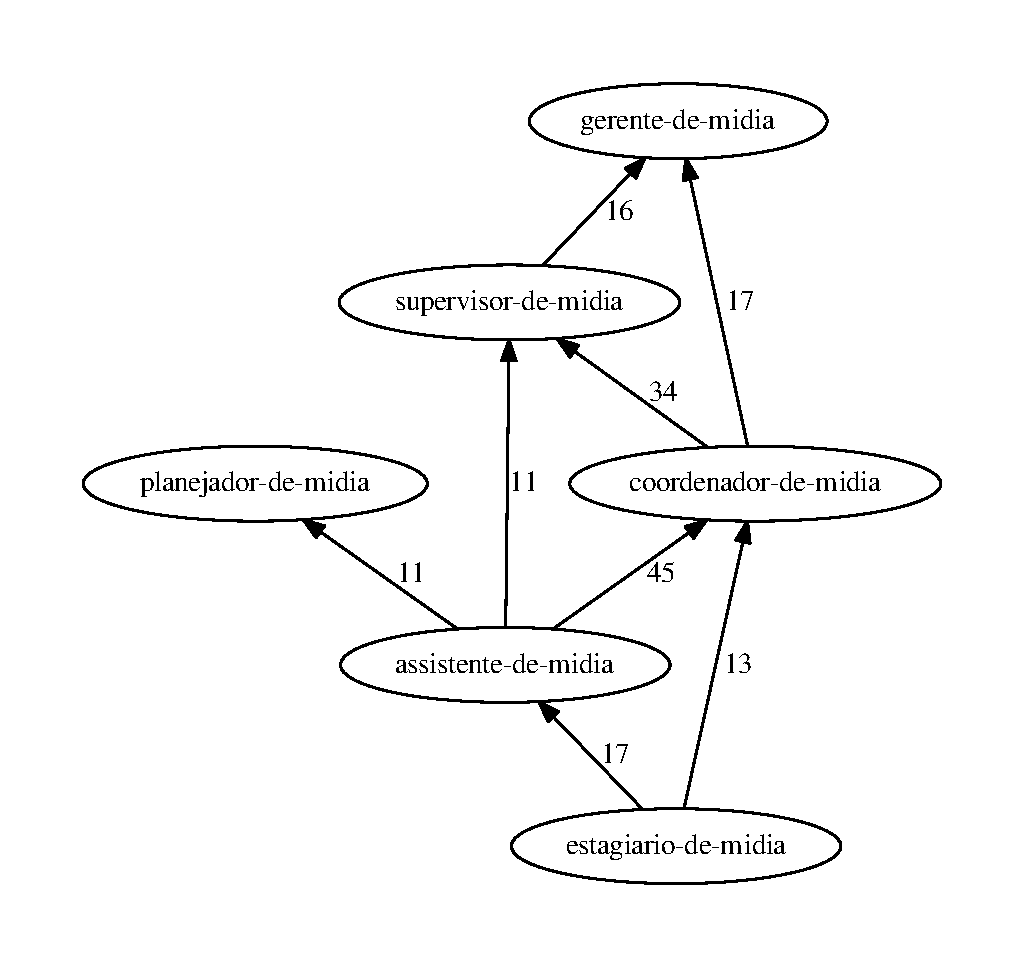
\includegraphics[scale=0.6]{cluster_23.pdf}
  \caption{Parte do MCar com ocupações relacionadas à carreira de mídia.}
  \label{fig:ex-mapa-midia}
\end{figure}

As ocupações no MCar foram definidas a partir de \textit{consenso} nos currículos. Como o título da ocupação é um campo em que o usuário digita livremente, assumiu-se que, se um grupo \enquote{suficientemente grande} de pessoas entra em acordo sobre uma certa nomenclatura, ela representa objetivamente uma ocupação. Essa abordagem é colocada de maneira implícita em ~\citeonline{Abbott1995-ft}, já \citeonline{Gunz2007-hr} a exploram para definir fronteiras de carreiras.

Uma das maiores dificuldades está em se definir o quanto um consenso precisa ser \enquote{suficientemente grande} para de fato existir uma ocupação. Para os fins desse trabalho, esse número foi obtido de forma experimental e empírica. Para isso, procurou-se o número mínimo de repetições exatas na grafia das ocupações de maneira que não fossem encontrados erros de digitação recorrentes, ou seja, que das ocupações criadas por consenso, nenhuma fosse resultado de erros frequentes de digitação. Esse número foi definido em 30 repetições, ou 10 transições com exatamente a mesma grafia em ambos os lados da transição.

Para a criação do MCar foram usados os currículos anonimizados de 10 milhões de usuários registrados no site VAGAS.com.br. A seleção de dados, bem como o processamento das informações, seguiu um procedimento conservador. Isso significa que as decisões tomadas em sua construção procuram minimizar os erros decorrentes da qualidade dos dados, mesmo que isso signifique trabalhar com uma quantidade menor deles. Utilizando o exemplo na Figura~\ref{fig:ex-mapa-midia}, isso significa que, provavelmente, muito mais do que 16 pessoas na base de dados fizeram a transição de \enquote{supervisor-de-midia} para a ocupação \enquote{gerente-de-midia}, porém, esses 16 são livres de erros e de subjetividade.

Da massa de currículos, apenas os atualizados no período entre 2011 e 2016 foram usados. Currículos em duplicação foram removidos usando o CPF como identificador; em caso de duplicação, apenas o currículo mais recente foi considerado. Na impossibilidade de se verificar a duplicação, como por exemplo, na ausência do CPF, o currículo também foi descartado.

Finalmente, algumas informações gerais foram extraídas dos currículos que passaram pelo processo acima e o restante das informações foi descartada, incluindo quaisquer maneiras de se identificar a pessoa descrita no currículo, garantindo a anonimidade do processo.

As informações extraídas são o sexo, último salário, graduação (se existente) ou escolaridade, e a sequência de ocupações pela qual o profissional passou com o título, descrição e período em que exerceu a ocupação.

O título da ocupação é um dos principais artefatos do MCar, é ele quem fornece a identidade para o nó. Como descrito acima, nos currículos, o título da ocupação é um campo de texto livre, ou seja, o usuário pode digitar o título sem restrições. Se por um lado isso permite a identificação de ocupações de nicho, novas ou que usem jargão de área; por outro isso significa que os títulos possuem erros de grafia, variações de gênero (como em \enquote{advogado} e \enquote{advogada} ou \enquote{moto boy} e \enquote{moto girl}), composição de múltiplas ocupações em um mesmo título (como \enquote{caixa/balconista}), abreviações e toda a gama de erros de interpretação possíveis.

As ocupações passam por um corretor ortográfico criado especificamente para esse trabalho, uma vez que um corretor tradicional não é capaz de identificar jargões de área como \enquote{enfermeiranda}, \enquote{rigger} ou \enquote{IRLA}.

Como exemplo, o dicionário do corretor possui cerca de 750 variações ortográficas que são traduzidas para o termo \enquote{auxiliar}, dentre eles, simples erros de omissão como \enquote{uxiliar}, até variações mais elaboradas como \enquote{ausciliar} e \enquote{alsilia}.

Após o trabalho de correção ortográfica, os títulos foram agrupados e contados. Especialistas da empresa verificaram os resultados dos maiores grupos para identificar anomalias, como ocupações com os títulos \enquote{sim}, \enquote{não} e \enquote{o mesmo}. Ocupações como essas foram excluídas do trabalho.

Finalmente, pares de ocupações foram gerados. Por exemplo, um currículo com a sequência de ocupações \enquote{saladeiro} $\to$ \enquote{chapeiro} $\to$ \enquote{cozinheiro} gera os pares \enquote{saladeiro} $\to$ \enquote{chapeiro} e \enquote{chapeiro} $\to$ \enquote{cozinheiro}.

Os pares foram agrupados e sua contagem se torna o peso de cada conexão na rede final. Nesse ponto do processo, cerca de 23 milhões de experiências profissionais dos currículos foram agrupadas em aproximadamente 7,5 mil ocupações distintas.

Finalmente, os pares de ocupações foram conectados entre si e a rede final foi construída e armazenada em um banco de dados de grafo. Um sistema online\footnote{Disponível em \url{http://www.vagas.com.br/mapa-de-carreiras}} disponibiliza as informações publicamente. Apesar de gratuito e de consulta pública, os dados do Mapa VAGAS da Carreira não são de uso livre. A empresa gentilmente cedeu os dados ao pesquisador para esse trabalho.

%===================================
\section{Grafos e Detecção de Comunidades} \label{sec:comunidades}
%===================================

Uma comunidade é um subgrafo com conexões mais \textit{coesas} entre seus nós do que com nós do restante do grafo. A palavra \enquote{coesão} aqui pode ser interpretada de várias maneiras. Para \citeonline{Ahn2010-uh,Evans2009-lq}, uma comunidade é definida quando o número de conexões internas do subgrafo é maior que o número de conexões que o conecta ao resto do grafo. Para \citeonline{Barabasi2016-rn,Newman2004-jg} a comunidade deve possuir uma densidade de conexões mais alta do que o esperado em uma rede aleatória equivalente. Para esses autores, o número de conexões é o fator determinante para a identificação da comunidade.

\citeonline{Rosvall2009-sd,Van_Dongen2000-qm}, por sua vez, trabalham a detecção de comunidades como a identificação de fluxos mais frequentes na rede. Assumindo que uma conexão representa um fluxo, comunidades possuem fluxo maior entre seus nós do que com nós fora da comunidade.

Essas abordagens distintas são aplicáveis a cenários diferentes. A densidade de conexões é mais adequada em redes onde a estrutura é importante, como, por exemplo, em uma rede social. Já em redes que representam fluxos, como circuitos ou redes de transporte, a segunda abordagem é mais atraente~\cite{Rosvall2009-sd}.

Para esse trabalho, a identificação de comunidades por fluxo é adequada por concepção. Como exposto na Seção~\ref{sec:carreira}, as fronteiras de carreira são definidas pelo consenso das movimentações profissionais: transições menos frequentes definem essas fronteiras.

Essa frequência é relativa ao fluxo entre os nós próximos: dez transições para uma ocupação como \enquote{Auxiliar Administrativo}, que possui dezenas de milhares de profissionais entrando e saindo, não tem a mesma importância que para \enquote{Assistente de Mídia} (Figura~\ref{fig:ex-mapa-midia}), em que essa dezena representa mais de 10\% das transições registradas.

O algoritmo Infomap (detalhado na Seção~\ref{sec:infomap}) utiliza \textit{random walkers} para identificar comunidades. Os caminhos em que eles circulam mais frequentemente são considerados como fazendo parte da mesma comunidade; por outro lado, caminhos raramente utilizados definem as fronteiras entre uma comunidade e outra, de maneira análoga à concepção de fronteiras de carreira de~\citeonline{Gunz2007-hr}.

Portanto, por analogia, a identificação de comunidades do algoritmo Infomap identifica fronteiras de carreiras em uma rede em que as conexões representam o fluxo de profissionais entre ocupações.

%===================================
\subsection{O Algoritmo Infomap} \label{sec:infomap}
%===================================

Segundo \citeonline{Grunwald2007-bt}, quaisquer regularidades em um conjunto de dados podem ser usadas para comprimi-los, ou seja, descrevê-los usando uma quantidade menor de símbolos. Quanto maior a regularidade, maior a compressão, dessa forma, dentre várias representações possíveis dos dados, a que apresentar maior compressão é também aquela que melhor identifica padrões nos dados. A Descrição de Comprimento Mínimo (\textit{Minimum Description Length}) é a disciplina que estuda essa relação.

O algoritmo Infomap aproveita essa dualidade entre detecção de padrões e compressão de dados para identificar padrões de fluxo em redes~\cite{Rosvall2009-sd}.

Para compreender o algoritmo, é preciso entender como um trajeto aleatório em uma rede é representado e como a Descrição de Comprimento Mínimo usa essa representação na detecção de comunidades.

Para isso, descreve-se o caminho que um \textit{random walker} faz em uma rede através da sequência de nós pelo qual ele passa. Por exemplo, assumindo uma rede com os nós $A$, $B$ e $C$, um caminho possível poderia ser descrito por $ABACBA$.

A Figura~\ref{fig:graph01} mostra um grafo regular, onde todos os nós possuem três vizinhos. Nesse tipo de rede, um \textit{random walker} ergódico (de caminho infinito) percorre todas as conexões o mesmo número de vezes. A Figura~\ref{fig:walk01} mostra um caminho aleatório passando por 800 nós.

\begin{figure}[ht]
  \centering
  \subfloat[][Rede regular] {
    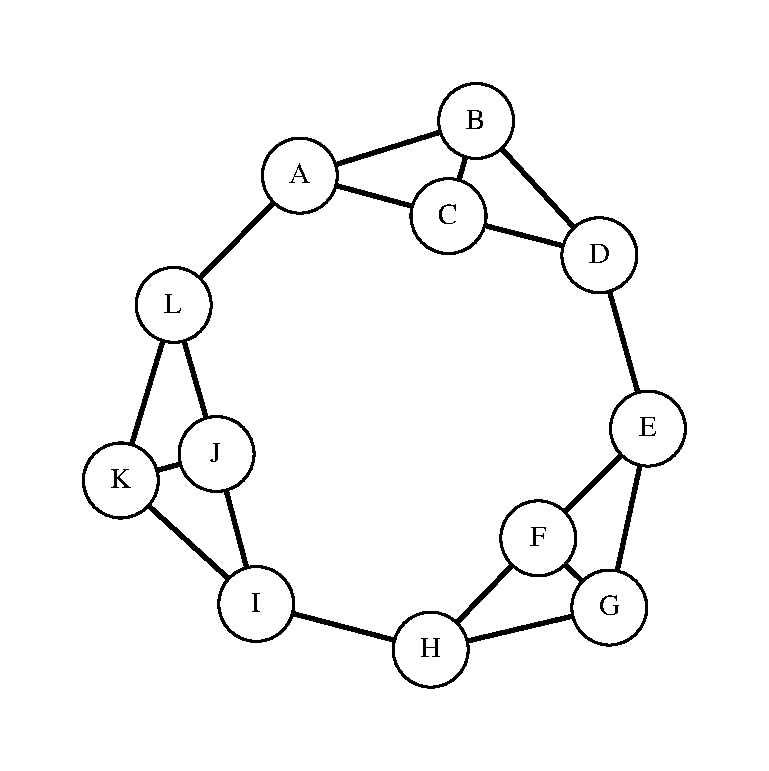
\includegraphics[scale=0.4]{graph01.pdf}
    \label{fig:graph01}
  }
  \subfloat[][Caminho na rede] {
    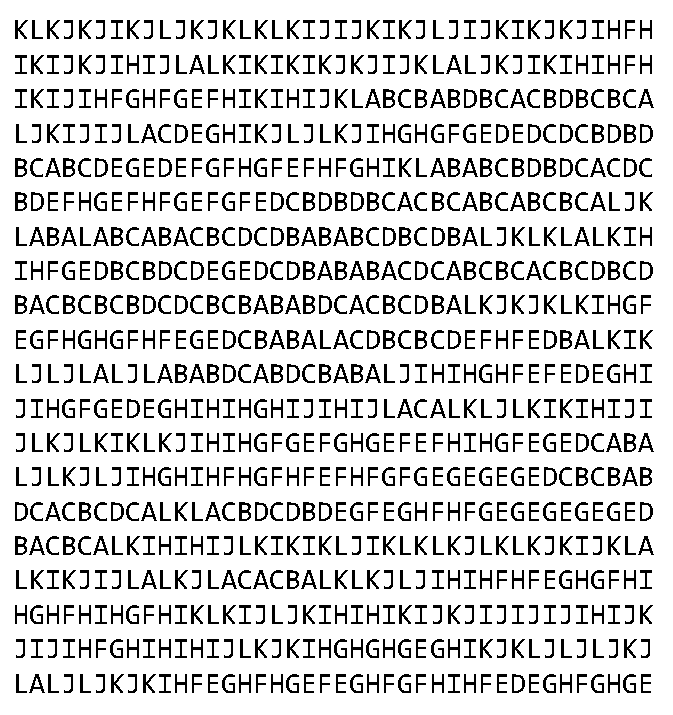
\includegraphics[scale=0.4]{graph01_path.pdf}
    \label{fig:walk01}
  }    
  \caption{Caminho de um \textit{random walker}}
\end{figure}

Apesar de ser uma rede regular, sua topologia faz com que o \textit{random walker} fique \enquote{preso} nos grupos formados pelos nós $ABCD$, $EFGH$ e $IJKL$; escapando esporadicamente de um para outro, onde circula até escapar novamente. Esses grupos são destacados na Figura~\ref{fig:graph02}. O caminho percorrido pelo \textit{walker} é exibido na Figura~\ref{fig:walk02}, dessa vez destacando os grupos por onde ele passa. As cores em ambas as figuras torna fácil perceber o comportamento do \textit{random walker}.

\begin{figure}[ht]
  \centering
  \subfloat[][Rede regular] {
    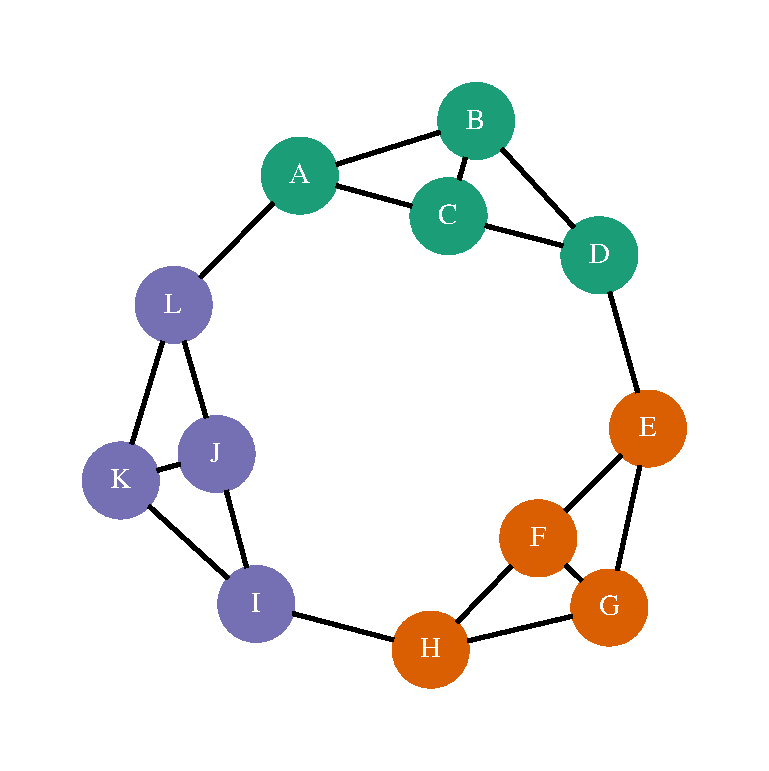
\includegraphics[width=0.4\linewidth]{graph02.pdf}
    \label{fig:graph02}
  }
  \subfloat[][Caminho na rede] {
    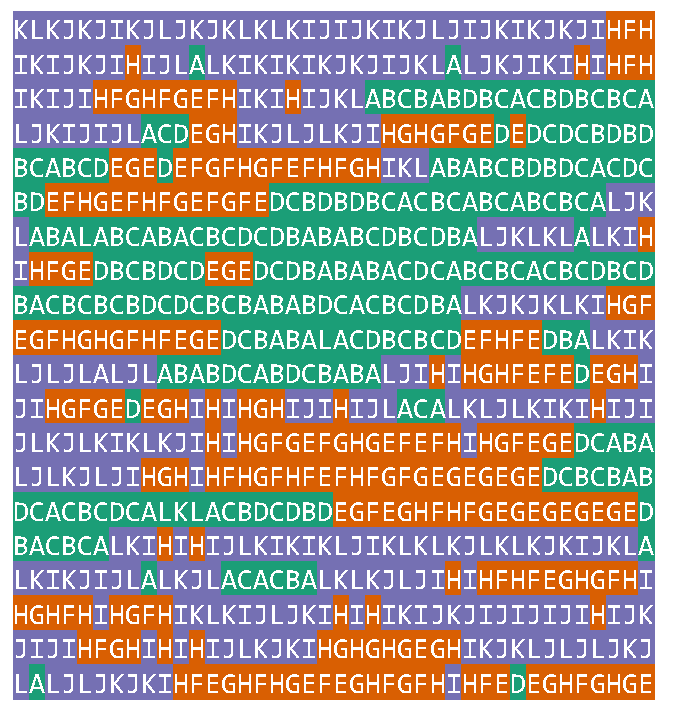
\includegraphics[width=0.4\linewidth]{graph02_path.pdf}
    \label{fig:walk02}
  }    
  \caption{Rede e caminho destacados}
\end{figure}

Se cada nó for representado por uma sequência de bits, podemos medir quanta informação é necessária para representar o caminho feito pelo \textit{random walker}. Usando a codificação de \citeonline{Huffman1952-ak} para nomear os nós de acordo com a Figura~\ref{fig:graph03}, o caminho da Figura~\ref{fig:walk01} é representado por 2880 bits.

Se a rede for dividida em grupos como anteriormente, e usarmos uma sequência única de bits para marcar quando o \textit{walker} entra ou sai de um grupo, podemos reaproveitar os códigos usados para descrever cada nó, compactando a informação necessária para representar o caminho. A Figura~\ref{fig:graph04} mostra os códigos para a entrada de cada grupo (\enquote{00}, \enquote{10} e \enquote{11}) e os códigos de saída de cada grupo (\enquote{111}), bem como os códigos dos nós. Com essa codificação, o caminho da Figura~\ref{fig:walk01} usa 1776 bits.

\begin{figure}[ht]
  \centering
  \subfloat[][Nós usando codificação de Huffman] {
    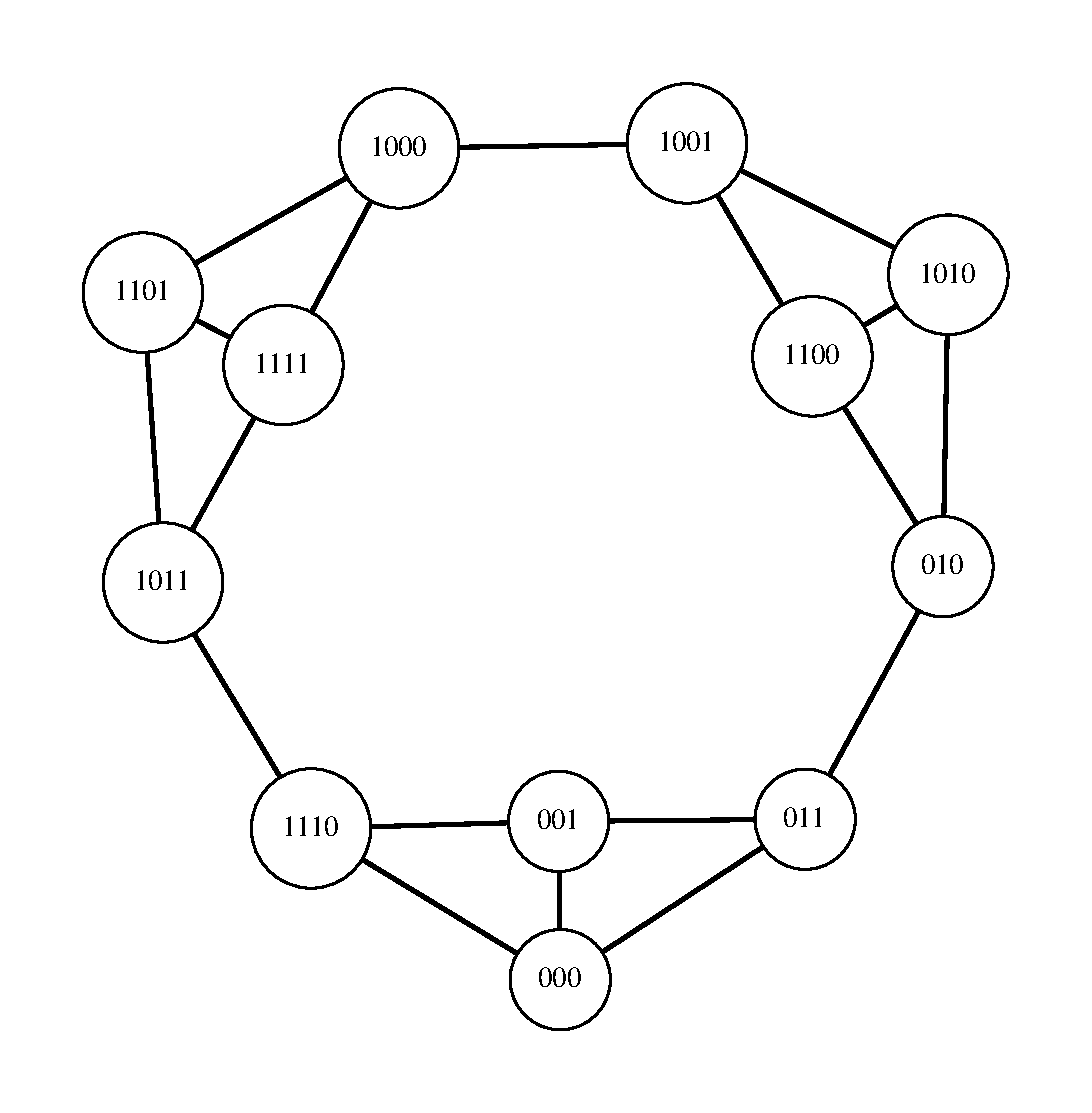
\includegraphics[width=0.4\linewidth]{graph03.pdf}
    \label{fig:graph03}
  }
  \subfloat[][Reaproveitamento de códigos] {
    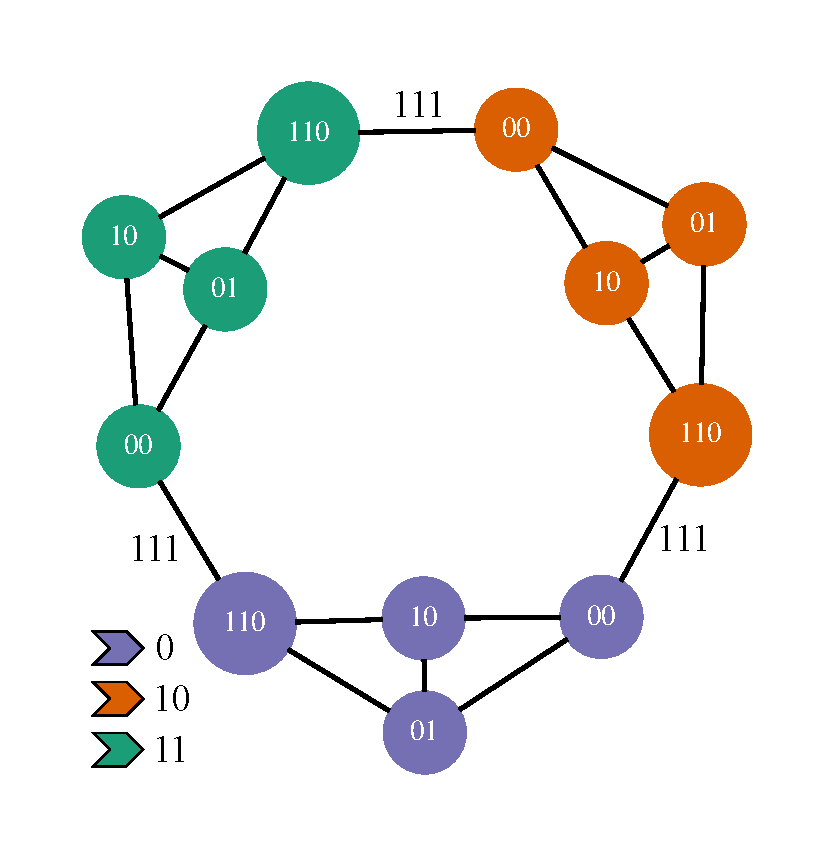
\includegraphics[width=0.4\linewidth]{graph04.pdf}
    \label{fig:graph04}
  }    
  \caption{Codificação dos nós}
\end{figure}

Portanto, o particionamento da rede em grupos onde os caminhos aleatórios podem ser representados da maneira mais compacta possível deve representar o melhor particionamento em relação ao fluxo.

A \enquote{Equação de Mapa}\footnote{\textit{Map Equation} no original}~\cite{Rosvall2009-sd} permite que se identifiquem as menores codificações possíveis para um determinado particionamento da rede sem a necessidade de se empregar \textit{random walkers} de fato. Com ela, a detecção de comunidades usando o fluxo como critério de coesão se reduz a um problema de otimização.

A Equação de Mapa é

\begin{equation*}
  L(\mathsf{M}) = q_\curvearrowright H(\mathcal{Q}) + \sum_{i=1}^{m}p^i_\circlearrowright H(\mathcal{P}^i)
\end{equation*}

Onde $L(\cdot)$ é o menor tamanho de codificação possível para representar um certo particionamento; $\mathsf{M}$ é o particionamento dos nós em $m$ comunidades; $i = 1, 2, \ldots, m$; $q_\curvearrowright$ é a probabilidade de um \textit{random walker} sair de uma comunidade e entrar em outra; $H(\mathcal{Q})$ (\textit{eta} em maiúsculo) é a média ponderada pela frequência do comprimento dos códigos usados para entrar nas comunidades; e $H(\mathcal{P}^i)$ também é a média do comprimento dos códigos ponderada pela frequência, mas dessa vez, daqueles usados na comunidade $i$; e finalmente $p^i_\circlearrowright$ é a probabilidade do \textit{walker} estar na comunidade $i$.

$H(X)$ é a equação que descreve a entropia da informação segundo uma certa distribuição de probabilidade $X$~\cite{Shannon1948-ic}. Ela se refere ao número mínimo de informação, usualmente na forma de bits, necessária para se representar uma mensagem.

A grosso modo, a Equação de Mapa pode ser descrita como \textit{o tamanho médio dos códigos para mudança de comunidade multiplicado pela probabilidade de troca de uma por outra, somada ao tamanho médio do código de cada comunidade multiplicado pela fração de tempo que o \textit{random walker} passa em cada uma}.

Existem variações da Equação de Mapa para detecção de comunidades sobrepostas~\cite{Viamontes_Esquivel2011-it} e hierárquicas~\cite{Rosvall2011-yi}. Este trabalho usa ambas as variações.

%% SE USAMOS AS VARIAÇÕES DA EQUAÇÃO DE MAPA, ENTÃO PRECISAMOS APRESENTÁ-LAS AQUI
% Ronie: vou tentar colocar de maneira bem resumida, pq cada uma é um trabalho bastante completo. Me avisa se ficar insuficiente, por favor.

%===================================
\subsection{Assortatividade} \label{sec:assortatividade}
%===================================

A assortatividade é uma medida de quão nós similares estão conectados entre si~\cite{Newman2003-jn}. A assortatividade de grau significa o quanto nós de grau similar são conectados entre si.

% Ronie: Preciso MUITO de uma ajuda com o matematiquês aqui :( A 'conta' tá certa, mas preciso de um jeito que fique compreensível. Ajuda, por favor!

Essa assortatividade em uma rede direcionada pode ser caracterizada pelo coeficiente de correlação de Pearson dos graus~\cite{Barabasi2016-rn}. Sendo $k_i^\leftarrow$ e $k_i^\rightarrow$  respectivamente os graus de entrada e saída do nó $i$, sendo $E$ o conjunto de conexões da rede, $e = (m, n) \mid e \in E$ as conexões de $E$, $m$ o vértice de onde $e$ sai e $n$ o vértice para onde $e$ aponta, definem-se os \textit{graus remanescentes} da conexão $e$ como

\begin{align*}
\delta_e^\leftarrow &= k_n^\leftarrow - 1
\\
\delta_e^\rightarrow &= k_m^\rightarrow - 1
\end{align*}

\begin{figure}[ht]
    \centering
    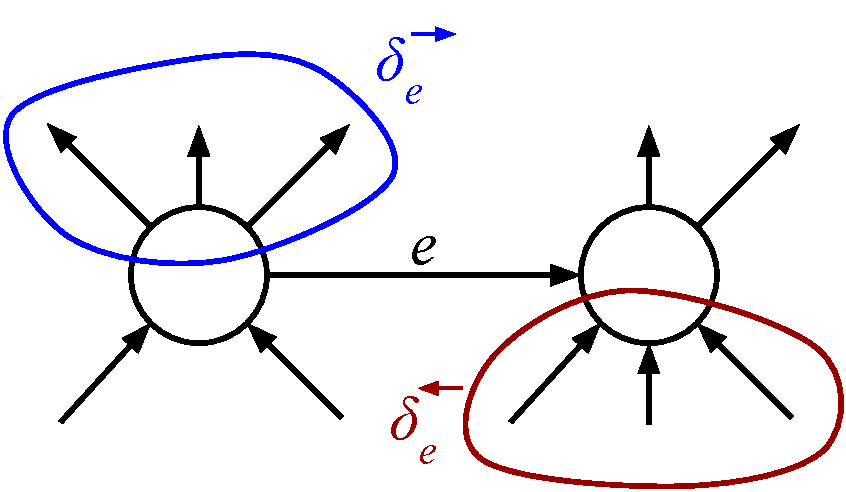
\includegraphics[scale=0.4]{remaining-degree.pdf}
    \caption{Graus remanescentes de entrada e saída da conexão $e$}
    \label{fig:remaining-degree}
\end{figure}

O \textit{grau remanescente} é o grau do nó, excetuando-se a conexão atual (Figura~\ref{fig:remaining-degree}). A correlação de Pearson $r$ dos graus é então definida por:

\begin{align*}
p &= \sum_{e \in E} \delta_e^\leftarrow \delta_e^\rightarrow
\\
q &= \frac{1}{|E|} \sum_{e \in E} \delta_e^\leftarrow
                                  \sum_{e \in E }\delta_e^\rightarrow
\\
\sigma^2_\leftarrow &= \sum_{e \in E} \left( \delta_e^\leftarrow \right)^2
            - \frac{1}{|E|} \left( \sum_{e \in E} \delta_e^\leftarrow \right)^2
\\
\sigma^2_\rightarrow &= \sum_{e \in E} \left( \delta_e^\rightarrow \right)^2
           - \frac{1}{|E|} \left( \sum_{e \in E} \delta_e^\rightarrow \right)^2
\\
r &= \frac{p - q}
                {\sqrt{ \sigma^2_\leftarrow } \sqrt{ \sigma^2_\rightarrow }}
\end{align*}

Em uma rede desassortativa, $r < 0$, o que significa que nós de maior grau tendem a se conectar com nós de menor grau. Esse tipo de rede é possui uma topologia de \enquote{eixo e raios} (\textit{hub and spokes}), onde os \textit{hubs} se conectam a muitos nós de grau mais baixo~\cite{Barabasi2016-rn}. A Figura~\ref{fig:ex-sobreposicao-ti} mostra um exemplo de uma rede em que predomina essa topologia.

%===================================
\subsection{Coeficiente de Agrupamento} \label{sec:coef-agrupamento}
%===================================

%% DEPOIS DE EXPLICAR O COEFICIENTE DE AGRUPAMENTO AINDA SERÁ PRECISO DIZER COMO O INFOMAP + A ASSORTATIVIDADE E O COEFICIENTE DE AGRUPAMENTO SÃO USADOS PARA DETECTAR COMUNIDADES
% Ronie: Na verdade, minha pretensão é usar essas duas medições para caracterizar a topologia das comunidades resultantes e talvez esse tópico e o anterior ficassem melhor em uma outra seção. O que estou observando (e quero números para comprovar) é que as comunidades tem uma topologia 'eixo e raios' (hub and spokes), ou seja, quase sempre algumas ocupações centrais conectam todas as outras da mesma comunidade, mas existem poucas conexões entre elas além da ocupação central. Confirmando isso, teríamos várias implicações interessantes que fogem ao escopo desse artigo. Por exemplo: essas são as ocupações mais críticas do mercado brasileiro, ou são as que possuem maior consenso, ou podemos criar um panorama geral criando um grafo só com elas e colapsando os 'raios'... e por aí vai. De qualquer forma, me parece uma boa maneira de caracterizar as comunidades.

%===================================
\section{Resultados e Conclusões} \label{sec:resultados}
%===================================

%% ESSA SEÇÃO DEVE COMEÇAR COM UMA DESCRIÇÃO DA METODOLOGIA EXPERIMENTAL, OU SEJA, DESCRIÇÃO DA BASE DE DADOS, QUAIS EXPERIMENTOS SERÃO REALIZADOS, QUAIS PARÂMETROS, O QUE SERÁ MEDIDO, ETC.

% Descrição dos dados:

A versão do MCar usada nesse trabalho é de fevereiro de 2017. Ela possui exatamente 7450 ocupações distintas e 90800 conexões.

A rede de ocupações possui a distribuição de grau exibida no gráfico de Pareto da Figura~\ref{fig:pareto-ocupacoes}. Ela possui uma grande concentração de conexões em poucos nós, formando \textit{hubs}. Os 25\% nós de maior grau são responsáveis por 89\% das conexões da rede. O nó de maior grau possui conexão com 6308 dos 7450 nós da rede, ou seja, ele conecta cerca de 85\% das ocupações.

\begin{figure}[htb]
  \centering
  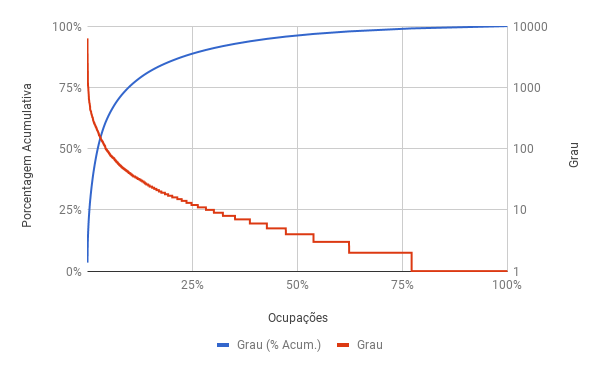
\includegraphics[width=0.9\linewidth]{pareto-ocupacoes.png}
  \caption{Gráfico de Pareto com a distribuição de grau. Os nós estão ordenados pelo grau de maneira decrescente no eixo horizontal, ocupações de grau maior estão à esquerda e ocupações de menor grau estão à direita. O eixo direito, em escala logarítmica, está associado à linha vermelha e representa o grau do nó. O eixo esquerdo está associado à linha azul e representa a somatória de todos os graus em porcentagem e qual a contribuição das ocupações à esquerda para essa totalização.}
  \label{fig:pareto-ocupacoes}
\end{figure}

Observando a Figura~\ref{fig:pareto-ocupacoes} é possível notar que quase $1/4$ das ocupações possui apenas uma conexão (1689 delas, $\approx$ 23\%). Independentemente do algoritmo de detecção de comunidades, esses nós serão levados a participar da mesma comunidade que seu parceiro. Essa configuração força o tamanho das comunidades para cima se elas contiverem um \textit{hub}. Por exemplo, mesmo que o nó de maior grau tenha preferência de conexão por outros nós de alto grau, ainda assim ele estaria conectado a pelo menos 8\% dos nós de grau 1. Ou seja, a menor comunidade possível que inclua o nó de maior grau possui ao menos aproximadamente 600 nós.

A presença de \textit{hubs} faz esperar que os grupos formados possuam um nó central altamente conectado, por onde passa o maior fluxo de profissionais.

% Procedimento:

Nos experimentos realizados, o algoritmo Infomap foi utilizado para encontrar o particionamento mais coeso do MCar em relação ao fluxo. Como exposto nas Seções~\ref{sec:carreira} e~\ref{sec:infomap}, esse particionamento é a própria definição de fronteiras de carreira.

O Infomap é bastante robusto quanto aos parâmetros utilizados, ou seja, mesmo grandes variações em seus parâmetros devem produzir resultados similares~\cite{Kawamoto2015-ha,Lambiotte2012-fp}. Por essa razão e para comparação com o trabalho de \citeonline{Viamontes_Esquivel2011-it}, os parâmetros padrões foram utilizados.

Para esse algoritmo, quanto maior a compressão da informação necessária para caracterizar o caminho do \textit{random walker}, melhor é o particionamento da rede~\cite{Rosvall2009-sd}.

O MCar foi testado em três variações: 
\begin{itemize}
\item Simples: consiste na detecção de comunidades em que cada nó pertence a apenas uma única comunidade. 
\item Hierárquica: procura-se detectar comunidades dentro de outras. 
\item Com sobreposição: permite-se que nós participem de mais de uma comunidade.
\end{itemize}

A variação com maior compressão revela a melhor caracterização de particionamento para aquela rede~\cite{Viamontes_Esquivel2011-it,Rosvall2011-yi}.

Os resultados de compressão para cada variação são apresentados na Tabela~\ref{tab:metodos}. É possível observar que as variações simples e hierárquica possuem quase a mesma compressão (os valores na tabela são aproximados), isso significa que o MCar não possui uma organização inerentemente hierárquica. Por outro lado, há um ganho expressivo de compressão quando se permite a sobreposição de comunidades, revelando que existem ocupações compartilhadas entre grupos profissionais diferentes.

% INTUITIVAMENTE UMA COMPRESSÃO MAIOR IMPLICA EM MENOS COMUNIDADES, PORÉM SUA TABELA MOSTRA O CONTRÁRIO, ASSIM COMO O TEXTO. DE ACORDO COM SUA EXPLICAÇÃO UMA MAIOR COMPRESSÃO IMPLICA EM MELHOR PARTICIONAMENTO E, PORTANTO, MAIS COMUNIDADES.
% Ronie: Aqui acho que preciso melhorar a explicação. Como tb não expliquei as variações hierárquicas e com sobreposição do Infomap estão também falta uma peça do quebra cabeças. A compressão dessa 'descrição do caminho do random walker' acaba criando um balanço entre quantidade de nós e de comunidades. Se não houverem 'gargalos' de fluxo, o random walker não fica 'preso' em um subgrafo e a melhor compressão acontece simplesmente por códigos mais curtos nos nós mais frequentes, sem divisão em comunidades. Por outro lado, quando existe um gargalo o random walker fica preso por um longo tempo de um lado ou de outro dele, nesse formato a melhor compressão acontece se cada 'prisão' reutilizar os códigos mais curtos e criarmos um outro código para passar de um lado para o outro do gargalo. O que está acontecendo na variação com sobreposição é que existem nós, ao invés de conexãos, que são fronteira entre as comunidades. Uma boa ilustração disso é o grafo 'gravata borboleta' com 5 nós e 6 conexões, nesse formato: ▷◁. Sem permitir sobreposição de comunidades, o nós central força os dois triângulos a pertencer em uma única comunidade. Permitindo a sobreposição, o nó central consegue participar de duas comunidades: ▷ e ◁. Se fosse uma rede com uma conexão entre os triângulos, desse jeito: ▷—◁, então o gargalo seria a conexão (não o nó) e o algoritmo que não permite sobreposição teria a melhor compressão.

\begin{table}
  \centering
  \begin{tabular}{@{} l r r @{}}
    \toprule
    Variação         & Compressão & Comunidades  \\
    \midrule
    Simples          & 14\%       & 123     \\
    Hierárquica      & 14\%       & 123     \\
    Com sobreposição & 44\%       & 926     \\
    \bottomrule
  \end{tabular}
  \caption{Métodos de detecção de comunidades e seus resultados. O \textit{Método} se refere ao tipo (variação) de particionamento. \textit{Compressão} significa qual a compressão obtida pelo Infomap em relação a uma rede sem particionamento. \textit{Partições} é o número de partições resultantes.}
  \label{tab:metodos}
\end{table}

\citeonline{Viamontes_Esquivel2011-it} apresentam um exemplo intuitivo do significado dessa sobreposição. Transposto para a realidade do MCar, uma ocupação que pertence a mais de uma comunidade significa que os profissionais que transitam por ela, em sua maioria, voltam aos seus grupos de origem ao invés de migrarem para outros. Não fosse dessa forma, esses grupos conectados seriam considerados como um conjunto único de ocupações pelo algoritmo.

Existem duas explicações possíveis. A primeira é que essas ocupações são \textit{homônimas} e portanto distintas, o que significa que há uma fronteira entre elas. A segunda é que essas ocupações são similares, mas fatores não especificados dificultam a transição de um grupo para outro. Novamente, isso indica uma fronteira de carreira, ainda que mais fraca.

Em qualquer uma dessas interpretações, as ocupações que participam de mais de uma comunidade revelam uma fronteira.

Os resultados obtidos foram comparados com o trabalho de \citeonline{Viamontes_Esquivel2011-it} para obter uma perspectiva mais ampla sobre o significado da compressão (Tabela~\ref{tab:comparativo}). É possível observar que o MCar é a rede que mais se beneficia de uma estrutura que permite sobreposição de comunidades, apesar de, comparativamente, ter uma estrutura modular comparável às outras redes do trabalho. Essa observação reforça a conclusão de que o particionamento com sobreposição melhor representa a estrutura do MCar.

\begin{table}
  \centering
  \begin{tabular}{@{} l r r r r r @{}}
    \toprule
                                           &      &          & \multicolumn{2}{c}{Compressão} & \\
    \cmidrule(r){4-5}
    Rede                                   & Nós  & Conexões & Simples & $\Delta$ Sobr.       & $N_{\text{sobr}}/N$ \\
    \midrule
    \rowcolor{yellow!25} Mapa de Carreiras & 7450 & 90800    & 14\%    & 30\%                 & 11\% \\
    Estradas Europeias                     & 1018 & 1274     & 46\%    & 10\%                 & 36\% \\
    Grade de Energia Leste dos EUA         & 4941 & 6994     & 53\%    & 8\%                  & 28\% \\
    Doenças Humanas                        & 516  & 1188     & 46\%    & 3\%                  & 15\% \\
    Coautoria de Artigos                   & 552  & 1317     & 49\%    & 2\%                  & 15\% \\
    Rotas Aéreas                           & 3618 & 14142    & 31\%    & 1\%                  & 14\% \\
    Blogs Políticos (EUA)                  & 1222 & 16714    & 4\%     & < 1\%                & 6\% \\
    Blogs Políticos (Suécia)               & 855  & 10315    & < 1\%   & < 1\%                & 5\% \\
    Rede Neural \textit{C. elegans}        & 297  & 2345     & 1\%     & < 1\%                & 3\% \\
    \bottomrule
  \end{tabular}
  \caption{Comparativo da estrutura do Mapa de Carreiras (em destaque) com outras redes~\cite{Viamontes_Esquivel2011-it}. \textit{Compressão Simples} se refere à compressão que o Infomap obteve no melhor particionamento simples da rede (sem sobreposição ou hierarquia de partições). \textit{Compressão $\Delta$ Sobr.} se refere ao ganho na compressão obtido pela sobreposição de partições em relação à compressão simples. $N_{\text{sobr}}/N$ é a proporção de nós que participam em mais de uma comunidade em relação ao total de nós.}
  \label{tab:comparativo}
\end{table}

A distribuição de tamanho das comunidades resultantes da partição com sobreposição está na Figura~\ref{fig:pareto-comunidades}. A maior parte das comunidades (mais de 75\% delas) possui apenas uma ocupação, representando cerca de 8\% das ocupações totais.

O tamanho das comunidades decresce rapidamente, 15\% das maiores comunidades (cerca de 135) englobam 90\% das ocupações, enquanto a maior comunidade possui sozinha cerca de $1/4$ das ocupações. Essa observação condiz com a expectativa de grandes comunidades impulsionadas pela presença de \textit{hubs}.

Apesar do grande ganho de compressão em um particionamento que permite a sobreposição de comunidades, uma quantidade relativamente pequena de ocupações, cerca de 11\%, é compartilhada entre comunidades.

As comunidades com apenas uma ocupação possuem duas explicações. A primeira são nós que interconectam comunidades maiores, mas com pouco fluxo entre elas, de maneira insuficiente para pertencer a uma das comunidades ou para conectá-las entre si. A segunda explicação se dá pelo limite de resolução, como citado na Seção~\ref{sec:comunidades}.

%% A QUE RESOLUÇÃO VOCÊ SE REFERE NO PARÁGRAFO ACIMA?

No primeiro caso, esses nós solitários devem possuir ao menos grau dois e seus parceiros devem pertencer à comunidades distintas. Essa situação só acontece em cerca de 10\% dos casos (73 em 718), o que aponta que o limite de resolução afeta a detecção de comunidades nesse caso. \citeonline{Kawamoto2015-ha}, recomendam o uso de agrupamento hierárquico para diminuir os efeitos do limite de resolução. Entretanto, sua aplicação nesse caso resulta em um comportamento similar com cerca de 10\% dos nós solitários (74 de 726) conectando comunidades distintas.

As comunidades, em sua maioria, possuem topologia em que predomina a forma de estrela ou estrelas com múltiplos centros. Isso significa poucos \textit{hubs} conectando quase todos os outros nós. Esse formato é caracterizado por uma baixa assortatividade e baixo coeficiente de agrupamento. Ou seja, nós de alto grau conectados a nós de baixo grau e poucos vizinhos a um terceiro nó são conectados entre si.

%% PRECISAMOS MOSTRAR E DISCUTIR ALGUNS EXEMPLOS DE COMUNIDADES AQUI. VAMOS DEBATER SEUS COMENTÁRIOS ABAIXO E DEFINIR ALGUNS CAMINHOS PARA FECHARMOS O TRABALHO

\begin{figure}[htb]
  \centering
  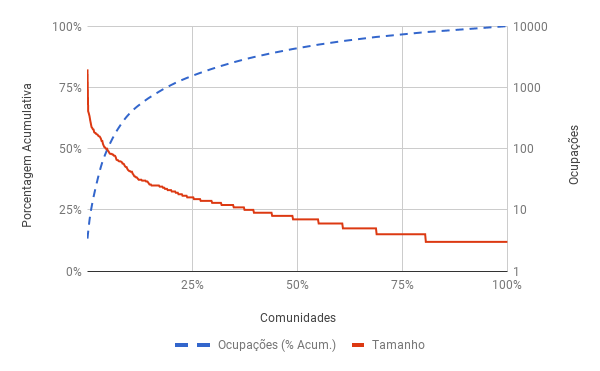
\includegraphics[width=0.9\linewidth]{pareto-comunidades.png}
  \caption{Gráfico de Pareto com a distribuição de tamanho das comunidades. As comunidades estão ordenadas pelo número de ocupações que contém, comunidades maiores estão à esquerda e comunidades menores à direita. O eixo direito, em escala logarítmica, está associado à linha vermelha e representa o tamanho da comunidade. O eixo esquerdo está associado à linha azul e representa o total de ocupações e qual a contribuição das comunidades à esquerda do ponto para ela.}
  \label{fig:pareto-comunidades}
\end{figure}


\begin{figure}[ht]
  \centering
  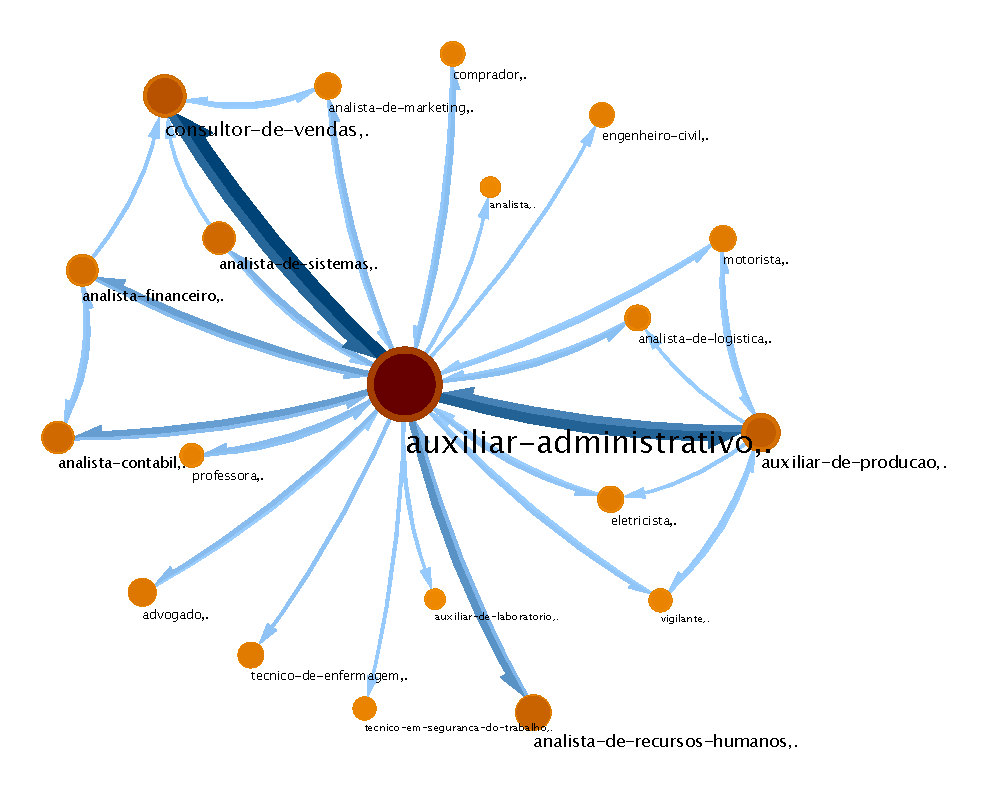
\includegraphics[width=0.9\linewidth]{ex-sobreposicao.pdf}
  \caption{20 maiores comunidades com as conexões de maior fluxo. A rede possui uma topologia entre \enquote{estrela} e \enquote{eixo e raios} (\textit{hub and spokes}). A adição de conexões de menor fluxo aproxima a topologia à de uma rede completa.  O tamanho do nó e das conexões se refere ao volume de fluxo que passa por eles.}
  \label{fig:ex-sobreposicao}
\end{figure}

\begin{comment}
A avaliação da qualidade possui sua cota da dificuldades. Por concepção, as fronteiras agrupam um conjunto de ocupações onde o indivíduo possui maiores chances de permanecer durante sua carreira. Uma análise possível seria o uso de \textit{random walkers} simulando pessoas se movimentando entre as ocupações. Entretanto, esse é o próprio conceito do algoritmo Infomap e essa \enquote{validação} apenas reproduziria o resultado do algoritmo. Portanto, o Infomap detecta as fronteiras de carreira pela própria \textit{definição} do conceito.

É importante observar que, apesar do algoritmo detectar as fronteiras de carreiras por definição, ele não fornece a dificuldade em se cruzar essa fronteira. O procedimento acima informa justamente essa dificuldade como uma forma de uma relação: pessoas que permanecem entre as fronteiras vs pessoas que as ultrapassam. A variação de parâmetros do algoritmo na verdade define o quão alta ou baixa é essa barreira entre os grupos de ocupações.

Outra forma de avaliação possível dos resultados é confrontar as fronteiras encontradas pelo algoritmo com carreiras de pessoas reais. A sequência de ocupações encontradas em currículos pode confirmar ou refutar as fronteiras. No entanto, a fonte de dados usada nesse trabalho é formada por milhões de currículos de pessoas reais, uma validação nesse sentido está fadada a reproduzir os resultados. O uso de outra base de currículos seria uma opção, porém, essa análise revelaria um possível viés da base ao invés da validação do procedimento.

Outra avaliação possível é verificar o significado das ocupações e confrontá-las com o conhecimento empírico de especialistas nas respectivas áreas. Por exemplo, entrevistar profissionais experientes de Tecnologia da Informação para verificar se as fronteiras encontradas correspondem ao seu conhecimento de movimentações na área. Por outro lado, como a fonte de dados usada possui um volume massivo de movimentações profissionais, a discordância entre o conhecimento empírico e o resultado revelaria um viés da base de dados usada ou uma limitação no conhecimento empírico, já que é baseado em uma amostra relativamente pequena em relação ao tamanho da base.

Finalmente, uma avaliação aplicável é verificar

Por concepção, os grupos resultantes sempre definem fronteiras de carreira. No entanto, é preciso avaliar se eles fazem sentido do ponto de vista social.

Para isso, é preciso analisar o significado de cada ocupação. Essa é uma tarefa que um computador (ainda) não é capaz

%% QUAL FOI O CRITÉRIO DE ESCOLHA DESSAS OCUPAÇÕES?
% Ronie: Na verdade, são todas as ocupações extraídas nessa versão. Mudei o texto, acha que ficou mais claro?

Como foi avaliado?

1 - Não há uma avaliação objetiva possível \\
2 - Pela própria definição de \enquote{fronteira de carreira}.
3 - Existem indícios de que as divisões fazem sentido: \\
 - A carreira de \enquote{mídia} foi separada pelo algoritmo, a direção predominante dos fluxos traz exatamente a sequência esperada de \enquote{evolução profissional}.

A aplicação do algoritmo Infomap resultou em 138 comunidades \textit{não-triviais}, onde uma comunidade \enquote{trivial}, nesse contexto, significa uma com apenas duas conexões, ou seja, três nós ou menos.

Permitindo que o algoritmo executasse agrupamento hierárquico, o primeiro nível possui apenas 3 grupos, um gigante composto por 6.722 nós, um segundo com 10 nós e o terceiro com 7 nós.

%% NÃO ENTENDI DE ONDE VEIO ESSE AGRUPAMENTO HIERÁRQUICO. POR QUE USÁ-LO, PARA QUE USÁ-LO?
% Ronie: essa pergunta me fez mudar o foco dos resultados, espero que para melhor :)

A existência de um grupo gigante indica que as carreiras são bastante diversificadas, fornecendo suporte ao conceito de \textit{Carreira sem Fronteiras}.

Subdividindo o grupo gigante, encontram-se 132 grupos com tamanhos exponencialmente crescentes. A Figura~\ref{fig:chart01} mostra os subgrupos por ordem decrescente de tamanho com o número de ocupações em escala logarítmica.

%% COMO FOI FEITA SUBDIVISÃO? POR QUE?

\begin{figure}[ht]
  \centering
  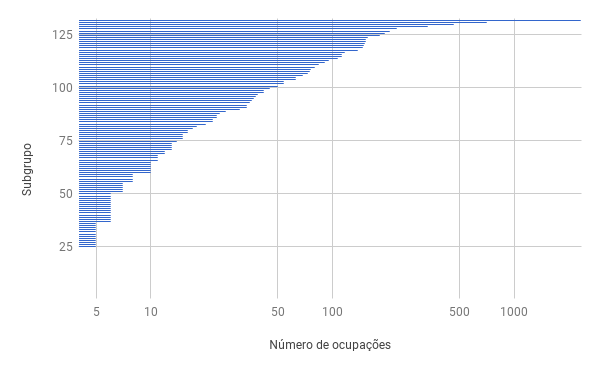
\includegraphics[width=0.7\linewidth]{chart01.png}
  \caption{Número de ocupações por subgrupo do grupo gigante}
  \label{fig:chart01}
\end{figure}

O maior desses subgrupos possui em sua maioria descrições de ocupações \textit{operacionais}, indicando que não existem fronteiras claras para esses profissionais. Esse resultado aponta para a capacitação técnica como uma das maiores barreiras na movimentação profissional. Como exemplo, as ocupações com maior grau de centralidade são exibidas na Tabela~\ref{tab:operacionais}.

\begin{table}[ht]
  \centering
  \begin{tabular}{c c}
    \toprule
    assistente-administrativo & auxiliar-administrativo \\
    atendimento & operador-de-caixa \\
    vendedor & recepcionista \\
    secretaria & jovem-aprendiz \\
    operador-de-telemarketing & caixa \\
    promotor-de-vendas & balconista \\
    consultor-de-vendas & auxiliar-de-producao  \\
    \bottomrule
  \end{tabular}
  \caption{Ocupações com maior centralidade de grau no maior subgrupo}
  \label{tab:operacionais}
\end{table}

Nesse trabalho, 898 ocupações aparecem em mais de um grupo. As ocupações compartilhadas por mais grupos são exibidas na Tabela~\ref{tab:multi-grupo}.

\begin{table}
  \centering
  \begin{tabular}{@{} l c l c @{}}
    \toprule
    Ocupação & Grupos & Ocupação & Grupos \\
    \midrule
    pesquisador & 20 &
    analista-comercial & 16 \\
    analista-planejamento & 15 &
    engenheiro-eletricista & 12 \\
    gerente-administrativo & 11 &
    assessor-tecnico & 11 \\
    docente & 11 &
    encarregado-geral & 11 \\
    gerente-operacao & 11 &
    inspetor-qualidade & 11 \\
    orcamentista & 11 &
    responsavel-tecnico & 11 \\
    socio-administrador & 10 &
    bolsista-iniciacao-cientifica & 10 \\
    \bottomrule
  \end{tabular}
  \caption{Ocupações que fazem parte de mais de um grupo}
  \label{tab:multi-grupo}
\end{table}

Muitos dos grupos menores resultam em Grafos Direcionados Acíclicos, revelando uma clara progressão de carreira. Outros são quase completamente acíclicos, com poucas conexões de pouco peso conectando nós em um aparente \enquote{retrocesso} na carreira. O significado dessas conexões é especulativo, mas uma pesquisa focada pode revelar se realmente seriam movimentos de retrocesso e suas motivações.

FIGURA - Exemplo de carreira \enquote{só pra frente}

FIGURA - Exemplo de carreira \enquote{pequena reversão}

Finalmente, o maior dos subgrupos, bem como alguns outros poucos, apresentam ciclos sem uma clara preferência. A Figura X mostra três das ocupações centrais do maior subgrupo, esse ciclo indica que algumas carreiras não são de fato uma sequência \textit{evolutiva} (em qualquer sentido possível, já que é um ciclo) como descrita por \citeonline{Arthur1989-rn}.

FIGURA X - Ciclo operacional

O aparecimento de grupos com progressão clara em oposição a grupos com a presença de ciclos fortes fornece combustível para discussões sobre modelos de carreira, em especial a noção de que \enquote{carreiras sem evolução} são comuns.

Finalmente, os próprios grupos resultantes possuem outras utilizações por si, já que representam os movimentos mais comuns nas ocupações brasileiras. Entre as possíveis aplicações eles podem ser usados como critério de classificação de ocupações; como plano de carreira baseado na progressão de menor barreira; ou como plano de treinamento de bases, já que as carreiras com progressão possuem claramente um ponto de partida; entre outros usos.
\end{comment}

%===================================
\section{Perspectivas Futuras}
%===================================

Os resultados desse trabalho fornecem indícios que suportam modelos de carreira, como o de \textit{Carreira sem Fronteiras}, ao mesmo tempo que indicam que eles não são abrangentes o suficiente para cobrir todos os segmentos profissionais. Carreiras sem Fronteiras, por exemplo, parecem ser mais apropriadas em ocupações operacionais do que para ocupações com maior exigência técnica. Análises localizadas podem comprovar ou refutar esse indício, bem como indicar quais modelos são mais adequados para quais segmentos.

Essa pesquisa contribui com suporte para um questionamento importante sobre a própria definição de carreira de que ela é um movimento \textit{evolutivo} na vida profissional de um indivíduo. A presença de ciclos fortes entre algumas ocupações sugere que existem carreiras onde não há progressão, mas sim uma movimentação lateral constante. Pesquisas orientadas podem refutar esse indício, uma vez que essa análise desconsidera os aspectos sociais e psicológicos da transição entre ocupações.

Algumas movimentações também sugerem que há retrocesso em alguns momentos da carreira. Entender se de fato são retrocessos e o que os motiva são linhas de pesquisa possíveis.

O MCar é uma fonte considerável de informação sobre o mercado de trabalho brasileiro. Outras pesquisas sobre profissões e carreira, em especial utilizando técnicas de Ciência de Redes, como \textit{motifs}, podem contribuir para uma melhor compreensão da dinâmica da movimentação profissional.

\newpage

\appendix

%===================================
\section{Exemplos de Grupos de Ocupações}
%===================================

\begin{figure}[h]
  \centering
  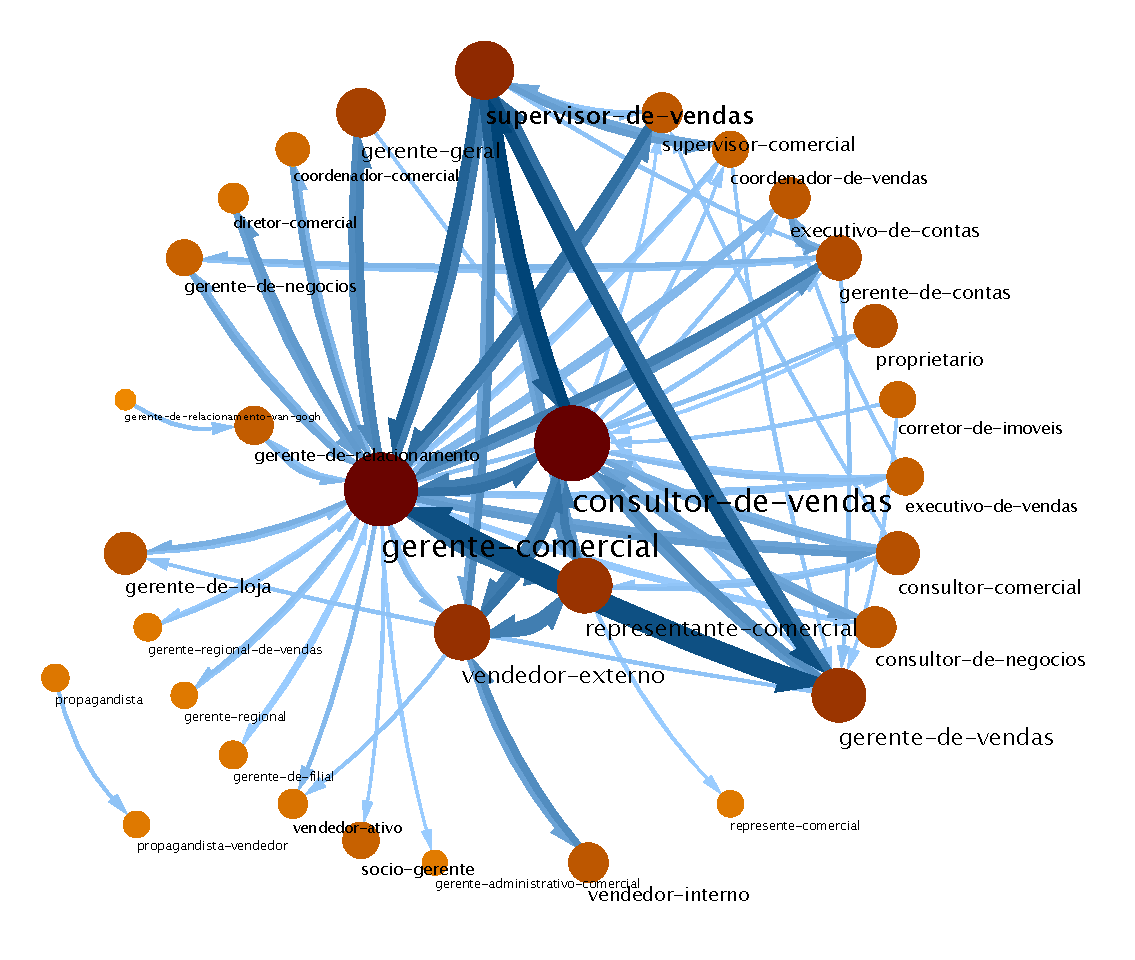
\includegraphics[width=0.7\linewidth]{ex-sobreposicao-consultor-de-vendas.pdf}
  \caption{20 maiores comunidades com as conexões de maior fluxo. A rede possui uma topologia entre \enquote{estrela} e \enquote{eixo e raios} (\textit{hub and spokes}). A adição conexões de menor fluxo aproxima a topologia à de uma rede completa.}
  \label{fig:ex-sobreposicao-vendas}
\end{figure}

\begin{figure}[h]
  \centering
  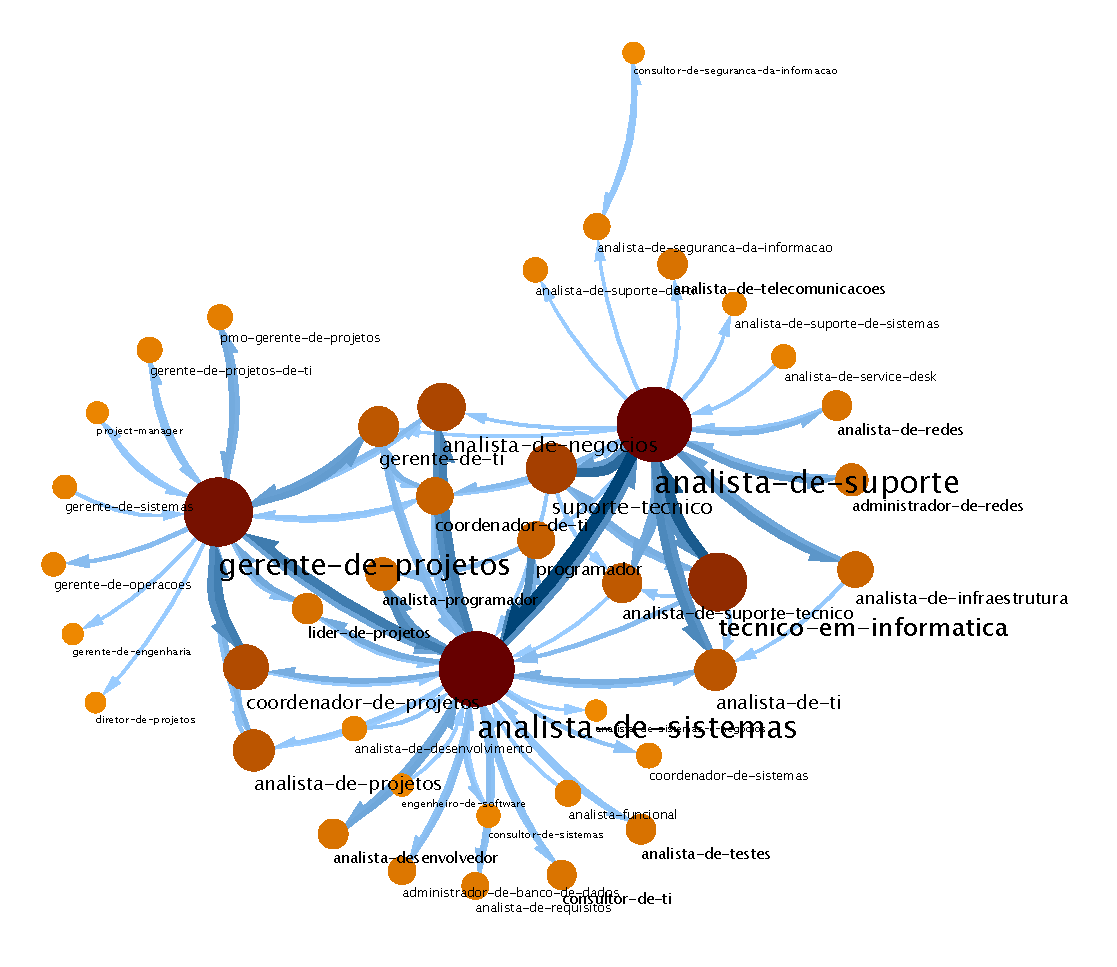
\includegraphics[width=0.7\linewidth]{ex-sobreposicao-analista-de-sistemas.pdf}
  \caption{20 maiores comunidades com as conexões de maior fluxo. A rede possui uma topologia entre \enquote{estrela} e \enquote{eixo e raios} (\textit{hub and spokes}). A adição conexões de menor fluxo aproxima a topologia à de uma rede completa.}
  \label{fig:ex-sobreposicao-ti}
\end{figure}

\begin{figure}[h]
  \centering
  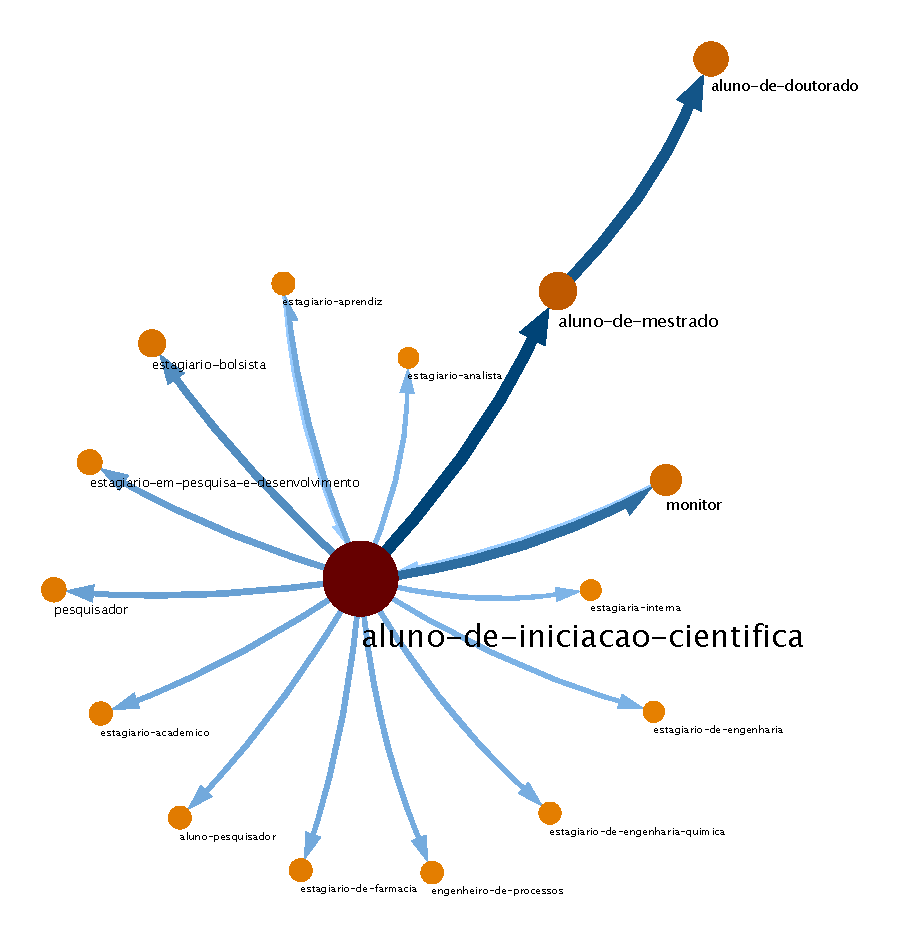
\includegraphics[width=0.7\linewidth]{ex-sobreposicao-aluno-iniciacao.pdf}
  \caption{20 maiores comunidades com as conexões de maior fluxo. A rede possui uma topologia entre \enquote{estrela} e \enquote{eixo e raios} (\textit{hub and spokes}). A adição conexões de menor fluxo aproxima a topologia à de uma rede completa.}
  \label{fig:ex-sobreposicao-ciencia}
\end{figure}

\newpage

\bibliography{main}
\end{document}
